\documentclass[../../../../main.tex]{subfiles}
\begin{document}

\begin{flushright}
\footnotesize\textit{【自動文字起こし・要確認】}
\end{flushright}

\noindent
\textbf{[解]} $1$ としておいて, $m, l, k \in \mathbb{N}$

\begin{center}
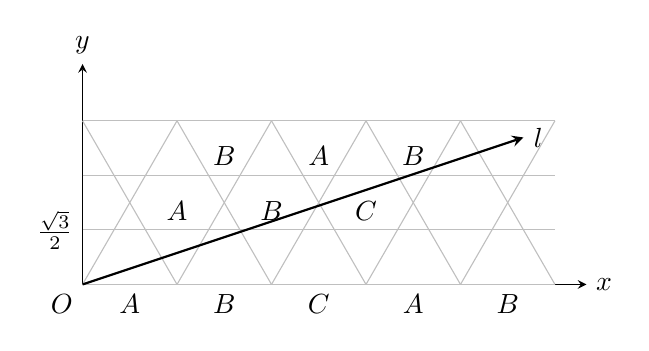
\begin{tikzpicture}[scale=0.8, >=stealth]
\draw[->] (0,0) -- (8,0) node[right] {$x$};
\draw[->] (0,0) -- (0,3.5) node[above] {$y$};
\node[below left] at (0,0) {$O$};

% Triangular tessellation lines
\foreach \i in {0,1,2,3} {
  \draw[gray!50] (0, \i*0.866) -- (7.5, \i*0.866);
}

\node[left] at (0, 0.866) {$\frac{\sqrt{3}}{2}$};

% Diagonal lines
\foreach \x in {0, 1.5, 3, 4.5, 6} {
  \draw[gray!50] (\x, 0) -- +({3*0.5}, {3*0.866});
  \draw[gray!50] (\x+1.5, 0) -- +({-3*0.5}, {3*0.866});
}

% Labels on vertices
\node[below] at (0.75,0) {$A$};
\node[below] at (2.25,0) {$B$};
\node[below] at (3.75,0) {$C$};
\node[below] at (5.25,0) {$A$};
\node[below] at (6.75,0) {$B$};

\node[above] at (1.5, 0.866) {$A$};
\node[above] at (3.0, 0.866) {$B$};
\node[above] at (4.5, 0.866) {$C$};

\node[above] at (2.25, 1.732) {$B$};
\node[above] at (3.75, 1.732) {$A$};
\node[above] at (5.25, 1.732) {$B$};

% Light ray line l
\draw[thick, ->] (0,0) -- (7, 2.333) node[right] {$l$};
\end{tikzpicture}
\end{center}

\noindent
上のように折り返して考えると, 光線は直線を進む. この時, 各頂点の座標は $\left(l, \frac{\sqrt{3}}{2}(2k)\right), \left(m+\frac{1}{2}, \frac{\sqrt{3}}{2}(2k-1)\right)$ と表せる. 又, $l$ がはじめてこれらの点とぶつかった時の点が, 到達する頂点である.

\bigskip

\noindent
(1) 光線 $l : y = \frac{\sqrt{3}}{4}x$ の時, 頂点は $\left(t, \frac{\sqrt{3}}{4}t\right)$ で表される. これがはじめて $\left(m+\frac{1}{2}, \frac{\sqrt{3}}{2}(2k-1)\right)$ の形になる時, $t = 2p \ (p \in \mathbb{N})$ が必要で, この時, $y$ 座標 $2p$ だから, $\min p = 2$ であり, もとめる頂点は B.

\bigskip

\noindent
(2) $l : y = \frac{\sqrt{3}}{6k+2}x$ の時, 頂点は $\left(t, \frac{\sqrt{3}}{6k+2}t\right)$ で表せる. これが $(m+\frac{1}{2}, \dots)$ の形になる時, $\frac{t}{3k+1} \in \mathbb{N}$ となることが必要で, $t = (3k+1)p \ (p \in \mathbb{N})$ と表せる. この時 $t \in \mathbb{Z}$ だから, $(m+\frac{1}{2}, \dots)$ より $\frac{t}{3k+1} = p$ が偶数であることが必要. これらをみたす $\min p = 2$ より, たどりつく座標は $(6k+2, \sqrt{3})$ である.

また $y$ 座標にある頂点は, その $x$ 座標を3でわって2あまると C だから, もとめる頂点は C. 又, 反射回数は, $l$ と各直線(AB, BC, CA)の共通点の数にひとしい. まず, $0 < y < \frac{\sqrt{3}}{2}$ の時, $(0 \le x < 3k+1), (t \le x < t+1) \ (t \in \mathbb{N})$ の区間で各々2本の直線と交わり, $0 < t \le 1$ の区間では1と交わるから, 計 $6k+1$ コ. 次に $y = \frac{\sqrt{3}}{2}$ の時, $x = 3k+1$ だから, ここで交わる直線は $y = \frac{\sqrt{3}}{2}$ のみで 1コ. 長くり $<\sqrt{3}$ の時も同様にして $6k+1$ コだから, あわせて
\[
12k+3 \text{ コ}
\]

\end{document}
